The stated goal of this task involved conducting an analysis to determine the optimal price increase to maintain current profit levels, under the expectation of a 25\% increase in operational costs. This analysis was carried out with an 8-function Python script. A detailed summary of each function, including its name, input parameters, and purpose, is presented in Table~\ref{tab:functions}.

This analysis was conducted under the assumption that, for each price increase considered, the bakery would also adjust its order quantity optimally, thereby minimizing losses due to under- or overstocking. Furthermore, profit deviations (whether above or below current levels) were treated symmetrically, as the primary goal was to maintain current profit levels rather than to maximize profit under the new cost burden.

The order of analysis started by first scaling the operational costs per store by a factor of 1.25, resembling the expected 25\% increase. After this, the expected percentage decrease in demand (\( rY \)) corresponding to a given percentage increase in price (\( rP \)) was calculated, using a formula (Fig.~\ref{fig:demand_drop}) provided by the bakery’s internal research team. Historical demand data for each store was then adjusted downward using a scaling factor of \( 1 - \frac{rY}{100} \), to simulate the impact of price sensitivity on consumer behavior. Based on the adjusted demand, the optimal order quantity (\( Q_{\text{new}} \)) was recalculated using the non-parametric function developed in the previous task. This step ensures that inventory decisions remain consistent with changes in decreased customer demand resulting from price increases, thereby providing a more realistic simulation of the relationship between pricing strategy and consumer behavior. To isolate the effect of the price increase on profitability from the confounding effect of also changing the demand, two parallel analyses were conducted: one assuming dynamic demand (where both demand and order quantity vary with \( rP \), reflecting a realistic scenario), and another with static demand (holding both demand and order quantity constant, to assess the direct financial impact of the cost and price changes in isolation).

\begin{figure}[h]
    \centering
    \caption{Demand Drop Formula (\( rY \))}
    \label{fig:demand_drop}
    \[
    rY = \left[ \left[ 1 + \exp\left(6 - \frac{rP}{10}\right) \right]^{-1} - 0.0025 \right] \times 100
    \]
\end{figure}

The next stage of the analysis involved comparing current profit levels (before the 25\% increase in operational costs and any price adjustments) with the expected profit levels resulting from different price increases (\( rP \)). Once again, two separate approaches were considered. The first analysis assumed that the bakery would continue its policy of uniform pricing across all store locations. In this scenario, the current profit level was calculated as the average profit across all stores, and each \( rP \) was evaluated by comparing this average to the average expected profit across all stores after the cost increase. Upon closer inspection, it became evident that while some stores remained highly profitable, others operated at a loss. These losses were effectively masked by the strong performance of the more profitable locations, leading to a misleading aggregate view.  Hence, assuming the bakery owners would like to keep each store profitable, a second approach was used. The second analysis ignored the uniform pricing assumption and evaluated each store independently. Here, the current profit for each store was individually compared to its expected profit under different \( rP \) values. This approach resulted in different optimal price increases per store and provides an alternative strategy for the bakery should it choose to abandon its same-price policy.

\renewcommand{\arraystretch}{1.4}
\begin{table}[H]
\begin{tabular}{|>{\columncolor{blue!20}}p{6cm}|p{5cm}|p{5cm}|}
    \hline
    \rowcolor{black!10}\textbf{Function name} & \textbf{Function Parameters} & \textbf{Function Purpose}  \\ \hline
    calculateDemandDrop & rP (percentage increase) & Computes the demand drop percentage from the price increase. \\ \hline
    adjustDemand & vY0 (original data set), rY (demand drop percentage) & Scales demand data by demand drop factor. \\ \hline
    nonparametricBootstrapCi & data (Demand data array), cr (Critical ratio (0–1)), alpha (Confidence level, default 0.05), B (Bootstrap iterations, default 1000) & Estimates quantile and confidence interval via bootstrap. \\ \hline
    calculateOptimalOrderQuantity & dfadjusted (Adjusted demand DataFrame), criticalratio (Critical ratio value) & Determines optimal order quantity per store using bootstrap. \\ \hline
    computeCurrentProfit & df (Demand data DataFrame), Q (Order quantity dictionary), c0 (Current cost dictionary), p0 (Current price dictionary), pL (Lowered price dictionary), cS (Shipping cost dictionary) & Calculates current profit for each store. \\ \hline
    computeNewProfit & dfadjusted (Adjusted demand DataFrame), Q (Order quantity dictionary), c1 (New cost dictionary), p1 (New price dictionary), pL (Lowered price dictionary), cS (Shipping cost dictionary) & Computes new profit with adjusted parameters. \\ \hline
    findOptimalPriceIncrease & Q (Initial order quantity dictionary), vY0 (Original demand DataFrame), c0 (Current cost dictionary), p0 (Current price dictionary), rprange (Tuple of start, stop, step for price range), criticalratio (Critical ratio value) & Finds best price increase to match current profit. \\ \hline
    plotProfitVsPriceIncrease & rpvalues (Array of price increases), profits (List of profit tuples), currentprofit (Tuple of current profits), bestrPperstore (Dictionary of optimal price increases) & Plots profit vs. price increase with optimal points. \\ \hline
\end{tabular}
\caption{Functions Overview for Price Sensitivity Analysis}
\label{tab:functions}
\end{table}

\newpage
\noindent\textbf{Analysis Results}
\medskip


Assuming static demand, with individualized store-level analysis, the results are visualized in Figure~\ref{fig:static}.

\begin{figure}[H]
    \centering
    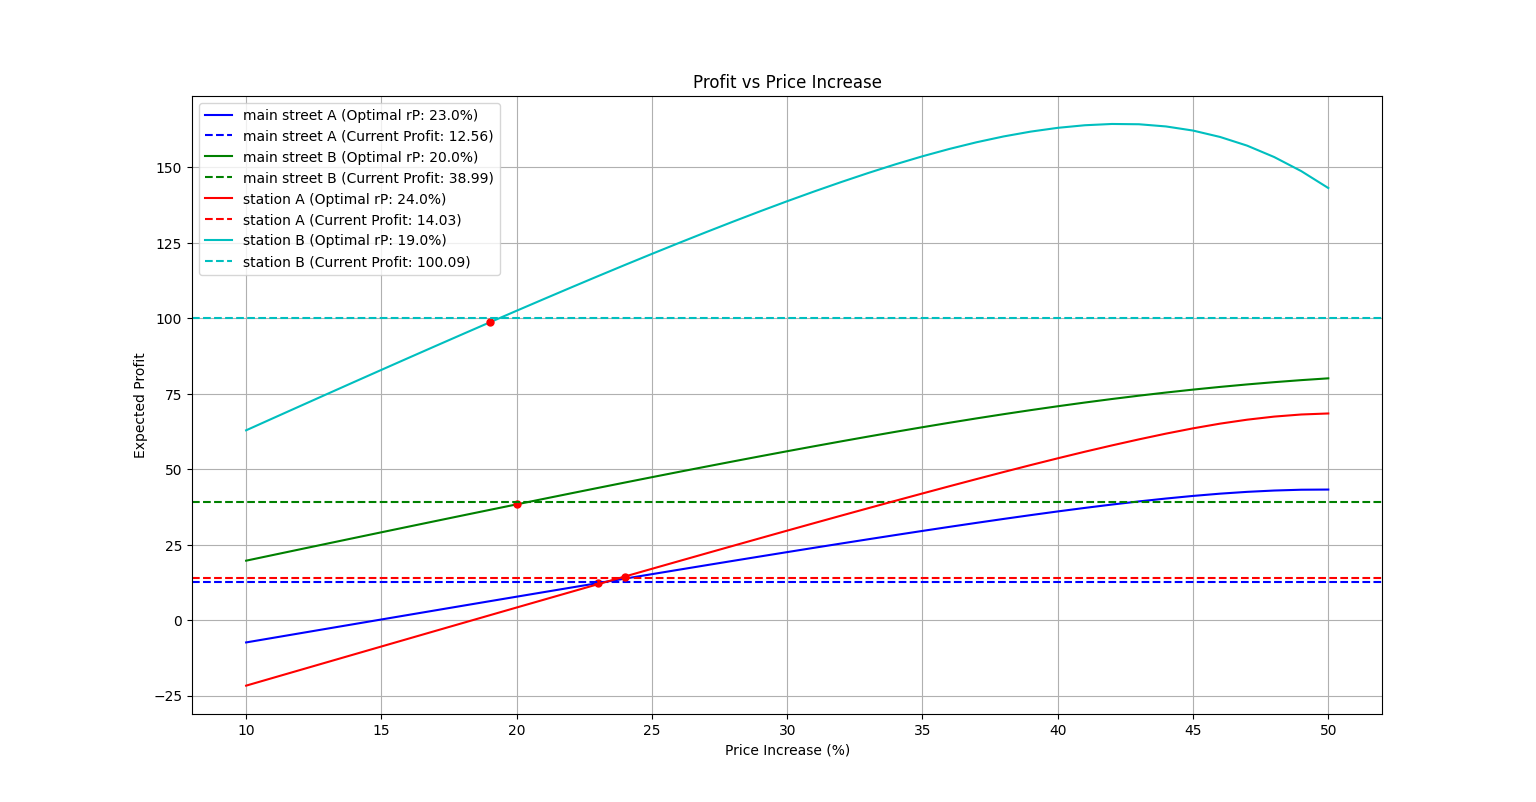
\includegraphics[width=0.85\textwidth]{Static Demand but individual stores.png}
    \caption{Profit vs. Price Increase under Static Demand (Individualized Stores)}
    \label{fig:static}
\end{figure}


The price increases required to maintain current levels of profitability are approximately 23.0\% for \textit{Main Street A}, 21.5\% for \textit{Main Street B}, 25.0\% for \textit{Station A}, and 19.0\% for \textit{Station B}. The graph indicates that beyond these optimal points, profit initially rises due to price increases outpacing the corresponding demand reduction. However, profit subsequently declines, implying that the model prioritizes \textbf{profit stability} over maximization.

\vspace{1em}

Assuming dynamic demand, with individualized store-level analysis, the results are shown in Figure~\ref{fig:dynamic}.

\begin{figure}[H]
    \centering
    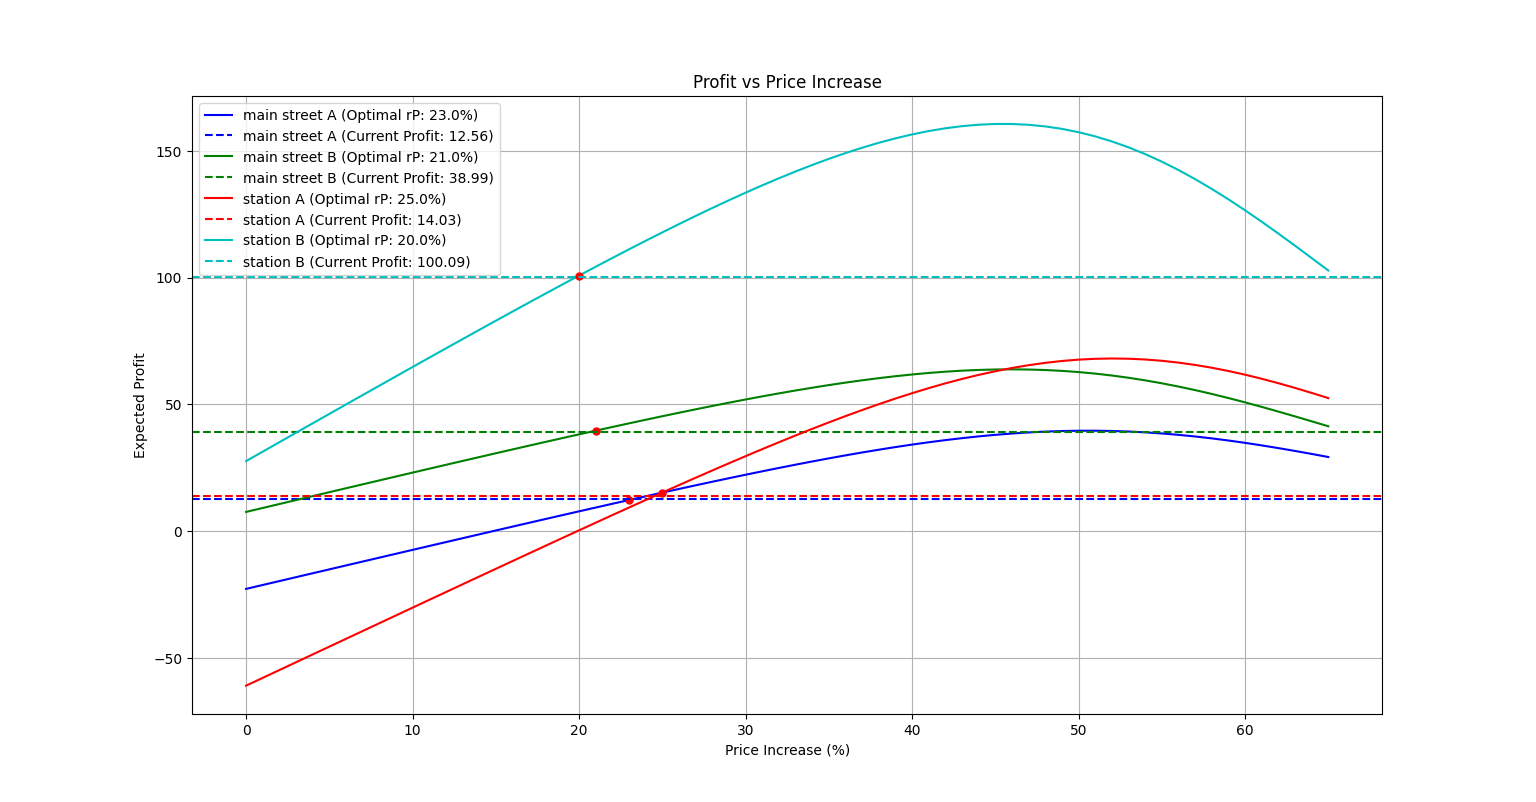
\includegraphics[width=0.85\textwidth]{Dynamic Demand.png}
    \caption{Profit vs. Price Increase under Dynamic Demand (Individualized Stores)}
    \label{fig:dynamic}
\end{figure}

The estimated price increases to maintain current production levels under dynamic demand are approximately 22.5\% for \textit{Main Street A}, 20.8\% for \textit{Main Street B}, 24.3\% for \textit{Station A}, and 18.5\% for \textit{Station B}. Once again, profits rise beyond the optimal price points, as the price increases initially outpace demand reductions, but then decline around 40--60\% due to more significant demand drops. As described in the methodology, optimal order quantities were dynamically adjusted using a nonparametric bootstrap approach. This model again emphasizes profit stability rather than maximization.

As stated in the methodology, the scenario assuming dynamic demand, with individualized store metrics, is the most realistic simulation that was run, and thus the results from Figure~\ref{fig:dynamic} would be the recommendation given to the store owners if they want to maintain current profit levels. The results, as seen, however, do not vary so significantly; this is thought to have happened due to the relatively tame effect a price increase has on demand reduction (26.64\% decrease for a 50\% price increase). Moreover, smaller price increases led to even milder effects:
\begin{itemize}
    \item 2\% increase → 0.05\% demand drop
    \item 10\% increase → 0.4\% demand drop
    \item 20\% increase → 1.54\% demand drop
    \item 30\% increase → 4.49\% demand drop
    \item 40\% increase → 11.67\% demand drop
\end{itemize}

This reinforces the conclusion that moderate price increases can effectively preserve profit levels without significantly harming demand.
